% Options for packages loaded elsewhere
\PassOptionsToPackage{unicode}{hyperref}
\PassOptionsToPackage{hyphens}{url}
%
\documentclass[
]{article}
\usepackage{amsmath,amssymb}
\usepackage{lmodern}
\usepackage{iftex}
\ifPDFTeX
  \usepackage[T1]{fontenc}
  \usepackage[utf8]{inputenc}
  \usepackage{textcomp} % provide euro and other symbols
\else % if luatex or xetex
  \usepackage{unicode-math}
  \defaultfontfeatures{Scale=MatchLowercase}
  \defaultfontfeatures[\rmfamily]{Ligatures=TeX,Scale=1}
\fi
% Use upquote if available, for straight quotes in verbatim environments
\IfFileExists{upquote.sty}{\usepackage{upquote}}{}
\IfFileExists{microtype.sty}{% use microtype if available
  \usepackage[]{microtype}
  \UseMicrotypeSet[protrusion]{basicmath} % disable protrusion for tt fonts
}{}
\makeatletter
\@ifundefined{KOMAClassName}{% if non-KOMA class
  \IfFileExists{parskip.sty}{%
    \usepackage{parskip}
  }{% else
    \setlength{\parindent}{0pt}
    \setlength{\parskip}{6pt plus 2pt minus 1pt}}
}{% if KOMA class
  \KOMAoptions{parskip=half}}
\makeatother
\usepackage{xcolor}
\IfFileExists{xurl.sty}{\usepackage{xurl}}{} % add URL line breaks if available
\IfFileExists{bookmark.sty}{\usepackage{bookmark}}{\usepackage{hyperref}}
\hypersetup{
  pdftitle={Experimental Design and Data Analysis - Assignment 1},
  pdfauthor={Group 75 - Sunny Soni, Maxine Palmen, Muska Neek},
  hidelinks,
  pdfcreator={LaTeX via pandoc}}
\urlstyle{same} % disable monospaced font for URLs
\usepackage[margin=1in]{geometry}
\usepackage{color}
\usepackage{fancyvrb}
\newcommand{\VerbBar}{|}
\newcommand{\VERB}{\Verb[commandchars=\\\{\}]}
\DefineVerbatimEnvironment{Highlighting}{Verbatim}{commandchars=\\\{\}}
% Add ',fontsize=\small' for more characters per line
\usepackage{framed}
\definecolor{shadecolor}{RGB}{248,248,248}
\newenvironment{Shaded}{\begin{snugshade}}{\end{snugshade}}
\newcommand{\AlertTok}[1]{\textcolor[rgb]{0.94,0.16,0.16}{#1}}
\newcommand{\AnnotationTok}[1]{\textcolor[rgb]{0.56,0.35,0.01}{\textbf{\textit{#1}}}}
\newcommand{\AttributeTok}[1]{\textcolor[rgb]{0.77,0.63,0.00}{#1}}
\newcommand{\BaseNTok}[1]{\textcolor[rgb]{0.00,0.00,0.81}{#1}}
\newcommand{\BuiltInTok}[1]{#1}
\newcommand{\CharTok}[1]{\textcolor[rgb]{0.31,0.60,0.02}{#1}}
\newcommand{\CommentTok}[1]{\textcolor[rgb]{0.56,0.35,0.01}{\textit{#1}}}
\newcommand{\CommentVarTok}[1]{\textcolor[rgb]{0.56,0.35,0.01}{\textbf{\textit{#1}}}}
\newcommand{\ConstantTok}[1]{\textcolor[rgb]{0.00,0.00,0.00}{#1}}
\newcommand{\ControlFlowTok}[1]{\textcolor[rgb]{0.13,0.29,0.53}{\textbf{#1}}}
\newcommand{\DataTypeTok}[1]{\textcolor[rgb]{0.13,0.29,0.53}{#1}}
\newcommand{\DecValTok}[1]{\textcolor[rgb]{0.00,0.00,0.81}{#1}}
\newcommand{\DocumentationTok}[1]{\textcolor[rgb]{0.56,0.35,0.01}{\textbf{\textit{#1}}}}
\newcommand{\ErrorTok}[1]{\textcolor[rgb]{0.64,0.00,0.00}{\textbf{#1}}}
\newcommand{\ExtensionTok}[1]{#1}
\newcommand{\FloatTok}[1]{\textcolor[rgb]{0.00,0.00,0.81}{#1}}
\newcommand{\FunctionTok}[1]{\textcolor[rgb]{0.00,0.00,0.00}{#1}}
\newcommand{\ImportTok}[1]{#1}
\newcommand{\InformationTok}[1]{\textcolor[rgb]{0.56,0.35,0.01}{\textbf{\textit{#1}}}}
\newcommand{\KeywordTok}[1]{\textcolor[rgb]{0.13,0.29,0.53}{\textbf{#1}}}
\newcommand{\NormalTok}[1]{#1}
\newcommand{\OperatorTok}[1]{\textcolor[rgb]{0.81,0.36,0.00}{\textbf{#1}}}
\newcommand{\OtherTok}[1]{\textcolor[rgb]{0.56,0.35,0.01}{#1}}
\newcommand{\PreprocessorTok}[1]{\textcolor[rgb]{0.56,0.35,0.01}{\textit{#1}}}
\newcommand{\RegionMarkerTok}[1]{#1}
\newcommand{\SpecialCharTok}[1]{\textcolor[rgb]{0.00,0.00,0.00}{#1}}
\newcommand{\SpecialStringTok}[1]{\textcolor[rgb]{0.31,0.60,0.02}{#1}}
\newcommand{\StringTok}[1]{\textcolor[rgb]{0.31,0.60,0.02}{#1}}
\newcommand{\VariableTok}[1]{\textcolor[rgb]{0.00,0.00,0.00}{#1}}
\newcommand{\VerbatimStringTok}[1]{\textcolor[rgb]{0.31,0.60,0.02}{#1}}
\newcommand{\WarningTok}[1]{\textcolor[rgb]{0.56,0.35,0.01}{\textbf{\textit{#1}}}}
\usepackage{graphicx}
\makeatletter
\def\maxwidth{\ifdim\Gin@nat@width>\linewidth\linewidth\else\Gin@nat@width\fi}
\def\maxheight{\ifdim\Gin@nat@height>\textheight\textheight\else\Gin@nat@height\fi}
\makeatother
% Scale images if necessary, so that they will not overflow the page
% margins by default, and it is still possible to overwrite the defaults
% using explicit options in \includegraphics[width, height, ...]{}
\setkeys{Gin}{width=\maxwidth,height=\maxheight,keepaspectratio}
% Set default figure placement to htbp
\makeatletter
\def\fps@figure{htbp}
\makeatother
\setlength{\emergencystretch}{3em} % prevent overfull lines
\providecommand{\tightlist}{%
  \setlength{\itemsep}{0pt}\setlength{\parskip}{0pt}}
\setcounter{secnumdepth}{-\maxdimen} % remove section numbering
\ifLuaTeX
  \usepackage{selnolig}  % disable illegal ligatures
\fi

\title{Experimental Design and Data Analysis - Assignment 1}
\author{Group 75 - Sunny Soni, Maxine Palmen, Muska Neek}
\date{2022-02-28}

\begin{document}
\maketitle

\hypertarget{question-1}{%
\subsection{Question 1}\label{question-1}}

\hypertarget{a}{%
\paragraph{\texorpdfstring{\textbf{1A}}{1A}}\label{a}}

Below, the measured waiting time in the waiting room of doctor's office
is given of 15 people. This waiting time is represented in a vector of
length 15, where the mean waiting time is a little more than 11 minutes.

\begin{Shaded}
\begin{Highlighting}[]
\NormalTok{waiting\_t }\OtherTok{\textless{}{-}} \FunctionTok{c}\NormalTok{(}\FloatTok{15.4}\NormalTok{, }\FloatTok{17.9}\NormalTok{, }\FloatTok{19.0}\NormalTok{, }\FloatTok{0.5}\NormalTok{, }\FloatTok{15.9}\NormalTok{, }\FloatTok{2.7}\NormalTok{, }\FloatTok{6.2}\NormalTok{, }\FloatTok{2.5}\NormalTok{, }\FloatTok{4.7}\NormalTok{, }\FloatTok{6.9}\NormalTok{, }\FloatTok{10.8}\NormalTok{, }\FloatTok{24.3}\NormalTok{, }\FloatTok{5.6}\NormalTok{, }\FloatTok{23.0}\NormalTok{, }\FloatTok{10.7}\NormalTok{)}
\NormalTok{mu\_t }\OtherTok{=} \FunctionTok{mean}\NormalTok{(waiting\_t)}
\FunctionTok{format}\NormalTok{(}\FunctionTok{round}\NormalTok{(mu\_t, }\DecValTok{3}\NormalTok{), }\AttributeTok{nsmall =} \DecValTok{3}\NormalTok{) }\CommentTok{\#rounding off to 3 decimals places }
\end{Highlighting}
\end{Shaded}

\begin{verbatim}
## [1] "11.073"
\end{verbatim}

There are several ways to check normality of the waiting time data, such
as a histogram, QQ-plot, Shapiro-wilk Test.The Histogram and QQ-plot are
graphical ways to check normality, and the Shapiro-wilk test is a
statistical test to check normality. In the Shapiro-wilk test, the
null-hypothesis claims that the sample data comes from a normal
distribution, and the alternative hypothesis claims that the sample data
does not come from normal distribution. This means that when the p-value
is above the confidence level of \(\alpha=0.05\), that the sample data
does come from normal distribution since the null hypothesis cannot be
rejected.

Below, we will perform all of these normality checks.

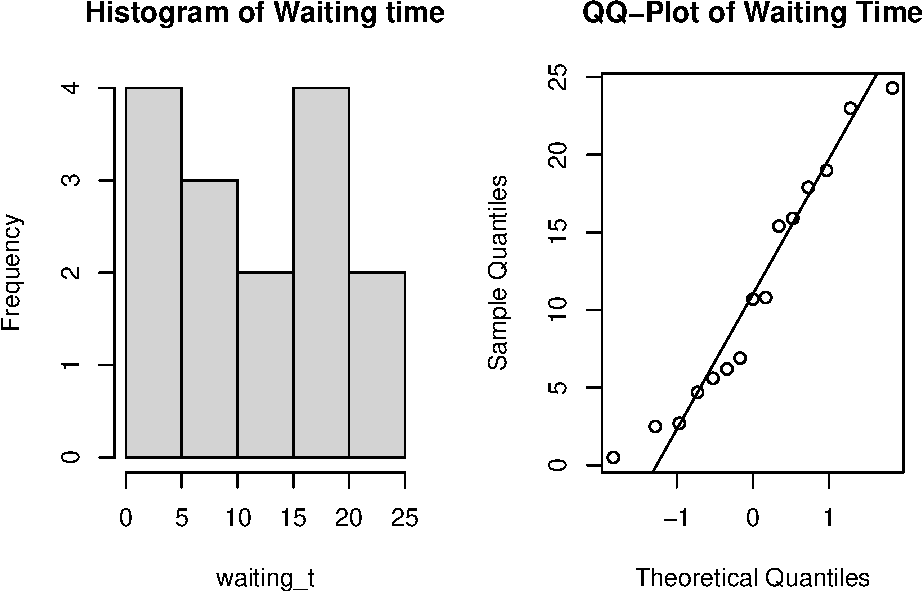
\includegraphics{assignment1_group75_final_files/figure-latex/unnamed-chunk-1-1.pdf}

According to the histogram, it seems that the waiting time data does not
come from a normal distribution. However, the sample size is very small,
which could influence this graphical test. The QQ-plot shows a quite
straight line of the sample data and therefore this could mean that the
sample data comes from normal distribution. To make the normality check
final, the Shapiro-Wilk test is performed to accept this assumption that
the sample data comes from normal distribution.

The result of the Shapiro-wilk test shows a p-value of 0.3. This means
that the data of the waiting time is normally distributed. To construct
a 97\%-CI, the following formula needs to be computed: mean(sample) +-
z*se where se is the standard error which is computed by: sd/sqrt(n)
where n is the sample size.

The upper and lower bound of 97\%-CI is {[}6.743, 15.403{]}

Bootstrap

\begin{Shaded}
\begin{Highlighting}[]
\NormalTok{B}\OtherTok{=}\DecValTok{1000}
\NormalTok{Tstar }\OtherTok{=} \FunctionTok{numeric}\NormalTok{(B)}
\ControlFlowTok{for}\NormalTok{(i }\ControlFlowTok{in} \DecValTok{1}\SpecialCharTok{:}\NormalTok{B)\{}
\NormalTok{  Xstar}\OtherTok{=}\FunctionTok{sample}\NormalTok{(waiting\_t, }\AttributeTok{replace=}\ConstantTok{TRUE}\NormalTok{)}
\NormalTok{  Tstar[i]}\OtherTok{=}\FunctionTok{mean}\NormalTok{(Xstar)\}}
\NormalTok{Tstar15}\OtherTok{=}\FunctionTok{quantile}\NormalTok{(Tstar, }\FloatTok{0.015}\NormalTok{)}
\NormalTok{Tstar985}\OtherTok{=}\FunctionTok{quantile}\NormalTok{(Tstar, }\FloatTok{0.985}\NormalTok{)}
\FunctionTok{sum}\NormalTok{(Tstar}\SpecialCharTok{\textless{}}\NormalTok{Tstar15)}
\FunctionTok{round}\NormalTok{(}\FunctionTok{c}\NormalTok{(}\DecValTok{2}\SpecialCharTok{*}\NormalTok{mu\_t}\SpecialCharTok{{-}}\NormalTok{Tstar985, }\DecValTok{2}\SpecialCharTok{*}\NormalTok{mu\_t}\SpecialCharTok{{-}}\NormalTok{Tstar15), }\DecValTok{3}\NormalTok{)}
\end{Highlighting}
\end{Shaded}

The 97\% bootstrap CI is {[}6.61, 14.86{]} The original CI was {[}6.743,
15.403{]}, which means that the bootstrap 97\%-CI and the original
97\%-CI do not differ much.

\hypertarget{b}{%
\paragraph{\texorpdfstring{\textbf{1B}}{1B}}\label{b}}

Claim: mean waiting time \textless{} 15 H0: mean waiting time
\textgreater= 15 H1: mean waiting time \textless{} 15 Since the data
comes from a normal distribution (see normality check at top of
document), a t-test can be used. We only have one data sample, and
therefor perform a one sample t-test.

The p-value for this one-sample t-test is 0.03, which means that the
null-hypothesis can be rejected and that the mean of the data sample
indeed is less than 15. The CI-interval for this t-test is
{[}-\(\infty\), 14.6{]}, which means that we can be 95\% sure that the
mean of the data sample lies within the CI-interval.

In the sign test we care about the median instead of the mean. Our
hypotheses H0 and H1 are still the same as in the one-sample t-test, but
instead of mean we use median. The hypothesized median is 15.

For this problem, the Wilcoxon signed rank test could also be performed.
This test needs a sample from a symmetric population and cares about the
median.

\hypertarget{c}{%
\paragraph{\texorpdfstring{\textbf{1C}}{1C}}\label{c}}

Compute powers of t-test and sign test

By comparing the power of the t-test and the sign-test, we can see that
the power of the t-test is higher than the power of the sign test.
Therefore, the t-test is a better test for this application. A reason
for this is that a t-test depends on normality and the data comes from a
normal distribution. So, therefore the t-test is more reliable.

\hypertarget{d}{%
\paragraph{\texorpdfstring{\textbf{1D}}{1D}}\label{d}}

The recovered confidence interval of the probability that a patient has
to wait longer than 15.5 minutes is {[}0.137, 0.53{]}, and this has a
confidence level of 89.39\%

\hypertarget{e}{%
\paragraph{\texorpdfstring{\textbf{1E}}{1E}}\label{e}}

Test of proportions H0: Proportion of long waiters of man is equal to
proportion of long waiters of woman Ha: Proportions are different

\begin{verbatim}
## Warning in prop.test(x = c(3, 2), n = c(7, 8)): Chi-squared approximation may be
## incorrect
\end{verbatim}

The p-value is 0.853, which is much larger than 0.05. Therefore, the
waiting time for man and woman are the same.

\hypertarget{question-2}{%
\subsection{Question 2}\label{question-2}}

\hypertarget{a-1}{%
\paragraph{\texorpdfstring{\textbf{2A}}{2A}}\label{a-1}}

The Kolmogorov-Smirnov normality test examines if variables are normally
distributed, which it is not because the data is exponentially
distributed. The Mann-Whitney U test is used to compare whether there is
a difference in the dependent variable for two independent groups. It
compares whether the distribution of the dependent variable is the same
for the two groups and therefore from the same population. The setting
needs to be symmetric, which our data is clearly not, therefore not
applicable. A t-test can only be used when comparing the means of two
groups (a.k.a. pairwise comparison), which is applicable.

\begin{Shaded}
\begin{Highlighting}[]
\CommentTok{\#check for normality, which they are not as seen in the following tests}
\NormalTok{clouds}\OtherTok{=}\FunctionTok{read.table}\NormalTok{(}\AttributeTok{file=}\StringTok{"clouds.txt"}\NormalTok{,}\AttributeTok{header=}\ConstantTok{TRUE}\NormalTok{)}
\NormalTok{seeded }\OtherTok{=}\NormalTok{ clouds[,}\DecValTok{1}\NormalTok{]}
\NormalTok{unseeded }\OtherTok{=}\NormalTok{ clouds [,}\DecValTok{2}\NormalTok{]}
\FunctionTok{par}\NormalTok{(}\AttributeTok{mfrow=}\FunctionTok{c}\NormalTok{(}\DecValTok{1}\NormalTok{,}\DecValTok{3}\NormalTok{))}
\FunctionTok{hist}\NormalTok{(seeded)}
\FunctionTok{boxplot}\NormalTok{(seeded)}
\FunctionTok{qqnorm}\NormalTok{(seeded)}
\FunctionTok{qqline}\NormalTok{(seeded)}
\end{Highlighting}
\end{Shaded}

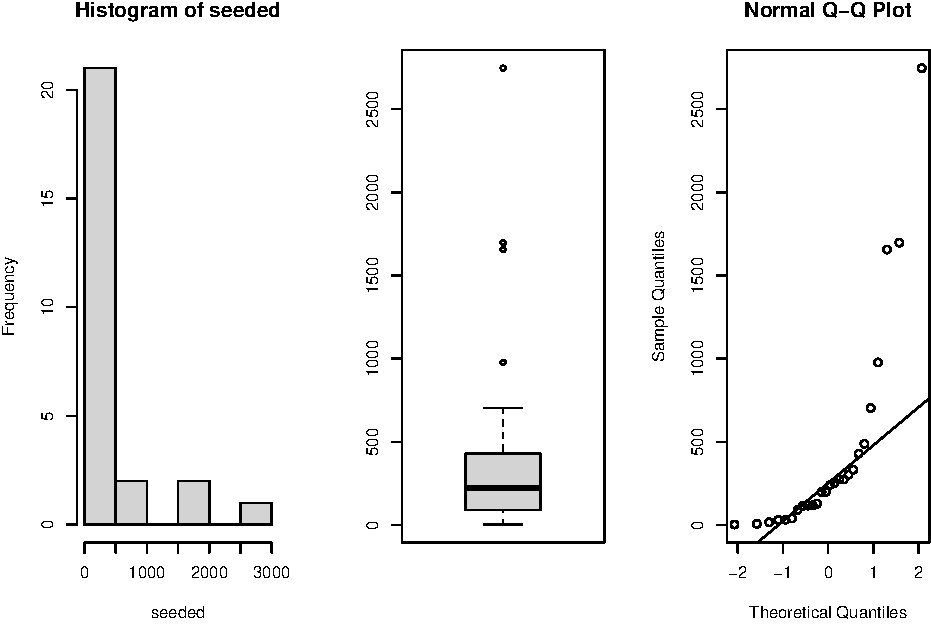
\includegraphics{assignment1_group75_final_files/figure-latex/unnamed-chunk-11-1.pdf}

\begin{Shaded}
\begin{Highlighting}[]
\FunctionTok{shapiro.test}\NormalTok{(seeded) }\CommentTok{\# extra test}
\end{Highlighting}
\end{Shaded}

\begin{verbatim}
## 
##  Shapiro-Wilk normality test
## 
## data:  seeded
## W = 0.656, p-value = 1.4e-06
\end{verbatim}

\begin{Shaded}
\begin{Highlighting}[]
\FunctionTok{hist}\NormalTok{(unseeded)}
\FunctionTok{boxplot}\NormalTok{(unseeded)}
\FunctionTok{qqnorm}\NormalTok{(unseeded)}
\FunctionTok{qqline}\NormalTok{(unseeded)}
\end{Highlighting}
\end{Shaded}

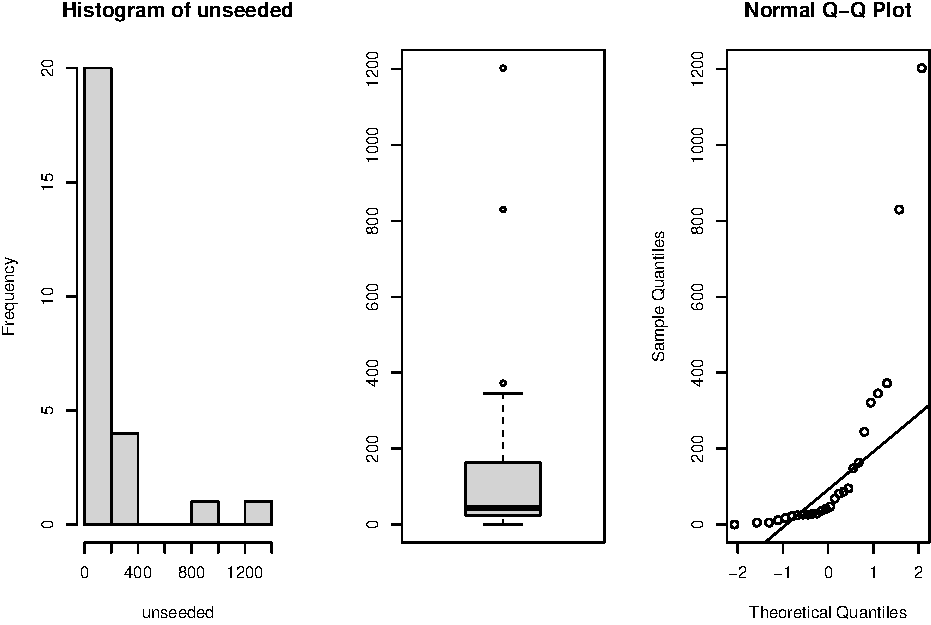
\includegraphics{assignment1_group75_final_files/figure-latex/unnamed-chunk-11-2.pdf}

\begin{Shaded}
\begin{Highlighting}[]
\FunctionTok{shapiro.test}\NormalTok{(unseeded) }\CommentTok{\#extra test}
\end{Highlighting}
\end{Shaded}

\begin{verbatim}
## 
##  Shapiro-Wilk normality test
## 
## data:  unseeded
## W = 0.603, p-value = 3.2e-07
\end{verbatim}

\begin{Shaded}
\begin{Highlighting}[]
\FunctionTok{t.test}\NormalTok{(seeded, unseeded)}
\end{Highlighting}
\end{Shaded}

\begin{verbatim}
## 
##  Welch Two Sample t-test
## 
## data:  seeded and unseeded
## t = 2, df = 33.9, p-value = 0.054
## alternative hypothesis: true difference in means is not equal to 0
## 95 percent confidence interval:
##   -4.7405 559.5859
## sample estimates:
## mean of x mean of y 
##    441.98    164.56
\end{verbatim}

\begin{Shaded}
\begin{Highlighting}[]
\FunctionTok{wilcox.test}\NormalTok{(seeded,unseeded)}
\end{Highlighting}
\end{Shaded}

\begin{verbatim}
## Warning in wilcox.test.default(seeded, unseeded): cannot compute exact p-value
## with ties
\end{verbatim}

\begin{verbatim}
## 
##  Wilcoxon rank sum test with continuity correction
## 
## data:  seeded and unseeded
## W = 473, p-value = 0.014
## alternative hypothesis: true location shift is not equal to 0
\end{verbatim}

\begin{Shaded}
\begin{Highlighting}[]
\FunctionTok{ks.test}\NormalTok{(seeded,unseeded)}
\end{Highlighting}
\end{Shaded}

\begin{verbatim}
## Warning in ks.test(seeded, unseeded): cannot compute exact p-value with ties
\end{verbatim}

\begin{verbatim}
## 
##  Two-sample Kolmogorov-Smirnov test
## 
## data:  seeded and unseeded
## D = 0.423, p-value = 0.019
## alternative hypothesis: two-sided
\end{verbatim}

\hypertarget{b-1}{%
\paragraph{\texorpdfstring{\textbf{2B}}{2B}}\label{b-1}}

Repeat the procedures from a) first on the square root of the values in
clouds.txt, then on the square root of the square root of the values in
clouds.txt. Comment on your findings.

Except for the t-test whereas the mean of both values are smaller, the
p-values are unchanged in the Mann-whitney and Kolmogorov-Smirnov test,
which is plausible and explainable when looking at their formulas,
because it takes the proportions into consideration. Therefore leading
to the same pvalue.

\begin{Shaded}
\begin{Highlighting}[]
\FunctionTok{t.test}\NormalTok{(}\FunctionTok{sqrt}\NormalTok{(seeded), }\FunctionTok{sqrt}\NormalTok{(unseeded))}
\end{Highlighting}
\end{Shaded}

\begin{verbatim}
## 
##  Welch Two Sample t-test
## 
## data:  sqrt(seeded) and sqrt(unseeded)
## t = 2.42, df = 43.4, p-value = 0.02
## alternative hypothesis: true difference in means is not equal to 0
## 95 percent confidence interval:
##   1.2021 13.0713
## sample estimates:
## mean of x mean of y 
##   17.0680    9.9313
\end{verbatim}

\begin{Shaded}
\begin{Highlighting}[]
\FunctionTok{wilcox.test}\NormalTok{(}\FunctionTok{sqrt}\NormalTok{(seeded),}\FunctionTok{sqrt}\NormalTok{(unseeded))}
\end{Highlighting}
\end{Shaded}

\begin{verbatim}
## Warning in wilcox.test.default(sqrt(seeded), sqrt(unseeded)): cannot compute
## exact p-value with ties
\end{verbatim}

\begin{verbatim}
## 
##  Wilcoxon rank sum test with continuity correction
## 
## data:  sqrt(seeded) and sqrt(unseeded)
## W = 473, p-value = 0.014
## alternative hypothesis: true location shift is not equal to 0
\end{verbatim}

\begin{Shaded}
\begin{Highlighting}[]
\FunctionTok{ks.test}\NormalTok{(}\FunctionTok{sqrt}\NormalTok{(seeded),}\FunctionTok{sqrt}\NormalTok{(unseeded))}
\end{Highlighting}
\end{Shaded}

\begin{verbatim}
## Warning in ks.test(sqrt(seeded), sqrt(unseeded)): cannot compute exact p-value
## with ties
\end{verbatim}

\begin{verbatim}
## 
##  Two-sample Kolmogorov-Smirnov test
## 
## data:  sqrt(seeded) and sqrt(unseeded)
## D = 0.423, p-value = 0.019
## alternative hypothesis: two-sided
\end{verbatim}

\hypertarget{c-1}{%
\paragraph{\texorpdfstring{\textbf{2C}}{2C}}\label{c-1}}

\(H_0\) : data is from a exponential distribution given that
p\textgreater{} 0.05 , also in KS-test, then the \(H_0\)can not be
rejected. Therefore, in conclusion of both tests the data is indeed from
an exponential distribution.

\begin{Shaded}
\begin{Highlighting}[]
\NormalTok{lambda }\OtherTok{=} \DecValTok{1} \SpecialCharTok{/} \FunctionTok{mean}\NormalTok{(seeded)}
\NormalTok{T1 }\OtherTok{=} \FunctionTok{mean}\NormalTok{(seeded)}
\NormalTok{z\_a }\OtherTok{=} \FunctionTok{qnorm}\NormalTok{(.}\DecValTok{975}\NormalTok{)}
\NormalTok{ci\_r }\OtherTok{=}\FunctionTok{mean}\NormalTok{(seeded)}\SpecialCharTok{+}\NormalTok{z\_a}\SpecialCharTok{*}\NormalTok{(}\FunctionTok{sd}\NormalTok{(seeded)}\SpecialCharTok{/}\FunctionTok{sqrt}\NormalTok{(}\DecValTok{26}\NormalTok{))}
\NormalTok{ci\_l }\OtherTok{=}\FunctionTok{mean}\NormalTok{(seeded)}\SpecialCharTok{{-}}\NormalTok{z\_a}\SpecialCharTok{*}\NormalTok{(}\FunctionTok{sd}\NormalTok{(seeded)}\SpecialCharTok{/}\FunctionTok{sqrt}\NormalTok{(}\DecValTok{26}\NormalTok{))}
\NormalTok{B}\OtherTok{=}\DecValTok{1000}
\NormalTok{Tstar}\OtherTok{=}\FunctionTok{numeric}\NormalTok{(B)}
\ControlFlowTok{for}\NormalTok{(i }\ControlFlowTok{in} \DecValTok{1}\SpecialCharTok{:}\NormalTok{B) \{}
\NormalTok{     Xstar}\OtherTok{=}\FunctionTok{rexp}\NormalTok{(seeded,lambda)}
\NormalTok{     Tstar[i]}\OtherTok{=}\FunctionTok{median}\NormalTok{(Xstar) \}}
\NormalTok{pl}\OtherTok{=}\FunctionTok{sum}\NormalTok{(Tstar}\SpecialCharTok{\textless{}}\NormalTok{T1)}\SpecialCharTok{/}\NormalTok{B; pr}\OtherTok{=}\FunctionTok{sum}\NormalTok{(Tstar}\SpecialCharTok{\textgreater{}}\NormalTok{T1)}\SpecialCharTok{/}\NormalTok{B; p}\OtherTok{=}\DecValTok{2}\SpecialCharTok{*}\FunctionTok{min}\NormalTok{(pl,pr)}
\NormalTok{pl;pr;p}
\end{Highlighting}
\end{Shaded}

\begin{verbatim}
## [1] 0.92
\end{verbatim}

\begin{verbatim}
## [1] 0.08
\end{verbatim}

\begin{verbatim}
## [1] 0.16
\end{verbatim}

\begin{Shaded}
\begin{Highlighting}[]
\FunctionTok{ks.test}\NormalTok{(seeded, }\FunctionTok{pexp}\NormalTok{(}\DecValTok{26}\NormalTok{, lambda))}
\end{Highlighting}
\end{Shaded}

\begin{verbatim}
## Warning in ks.test(seeded, pexp(26, lambda)): cannot compute exact p-value with
## ties
\end{verbatim}

\begin{verbatim}
## 
##  Two-sample Kolmogorov-Smirnov test
## 
## data:  seeded and pexp(26, lambda)
## D = 1, p-value = 0.29
## alternative hypothesis: two-sided
\end{verbatim}

\hypertarget{d-1}{%
\paragraph{\texorpdfstring{\textbf{2D}}{2D}}\label{d-1}}

Using an appropriate test, verify whether the median precipitation for
seeded clouds is less than 300. Next, design and perform a test to check
whether the fraction of the seeded clouds with the precipitation less
than 30 is at most 25\%.

\begin{Shaded}
\begin{Highlighting}[]
\FunctionTok{sum}\NormalTok{(seeded}\SpecialCharTok{\textless{}}\DecValTok{300}\NormalTok{) }
\end{Highlighting}
\end{Shaded}

\begin{verbatim}
## [1] 17
\end{verbatim}

\begin{Shaded}
\begin{Highlighting}[]
\FunctionTok{binom.test}\NormalTok{(}\DecValTok{17}\NormalTok{,}\DecValTok{26}\NormalTok{,}\AttributeTok{p=}\FloatTok{0.5}\NormalTok{) }\CommentTok{\#H0 is therefore not rejected, which means that at the median  precipitation for seeded clouds is less than 300 is indeed at the given median.  }
\end{Highlighting}
\end{Shaded}

\begin{verbatim}
## 
##  Exact binomial test
## 
## data:  17 and 26
## number of successes = 17, number of trials = 26, p-value = 0.17
## alternative hypothesis: true probability of success is not equal to 0.5
## 95 percent confidence interval:
##  0.44333 0.82786
## sample estimates:
## probability of success 
##                0.65385
\end{verbatim}

\begin{Shaded}
\begin{Highlighting}[]
\CommentTok{\#there are different way to check this whereas the first method is:}
\FunctionTok{quantile}\NormalTok{(seeded)}
\end{Highlighting}
\end{Shaded}

\begin{verbatim}
##       0%      25%      50%      75%     100% 
##    4.100   98.125  221.600  406.025 2745.600
\end{verbatim}

\begin{Shaded}
\begin{Highlighting}[]
\CommentTok{\#the binomial method could also be used: }
\FunctionTok{binom.test}\NormalTok{(}\DecValTok{17}\NormalTok{,}\DecValTok{26}\NormalTok{,}\AttributeTok{p=}\FloatTok{0.25}\NormalTok{, }\AttributeTok{alternative =} \StringTok{"l"}\NormalTok{)}
\end{Highlighting}
\end{Shaded}

\begin{verbatim}
## 
##  Exact binomial test
## 
## data:  17 and 26
## number of successes = 17, number of trials = 26, p-value = 1
## alternative hypothesis: true probability of success is less than 0.25
## 95 percent confidence interval:
##  0.00000 0.80604
## sample estimates:
## probability of success 
##                0.65385
\end{verbatim}

\begin{Shaded}
\begin{Highlighting}[]
\CommentTok{\#just as the propportion test}
\FunctionTok{prop.test}\NormalTok{(}\DecValTok{17}\NormalTok{,}\DecValTok{26}\NormalTok{,}\AttributeTok{p=}\FloatTok{0.25}\NormalTok{, }\AttributeTok{alt=}\StringTok{"l"}\NormalTok{)}
\end{Highlighting}
\end{Shaded}

\begin{verbatim}
## 
##  1-sample proportions test with continuity correction
## 
## data:  17 out of 26, null probability 0.25
## X-squared = 20.5, df = 1, p-value = 1
## alternative hypothesis: true p is less than 0.25
## 95 percent confidence interval:
##  0.0000 0.8017
## sample estimates:
##       p 
## 0.65385
\end{verbatim}

\hypertarget{question-3}{%
\subsection{Question 3}\label{question-3}}

\textbf{Loading the dataset}

\begin{Shaded}
\begin{Highlighting}[]
\NormalTok{dogs\_data }\OtherTok{=} \FunctionTok{read.table}\NormalTok{(}\StringTok{"dogs.txt"}\NormalTok{,}\AttributeTok{header=}\ConstantTok{TRUE}\NormalTok{)}
\NormalTok{Isofluorane }\OtherTok{=}\NormalTok{ dogs\_data}\SpecialCharTok{$}\NormalTok{isofluorane}
\NormalTok{Halothane }\OtherTok{=}\NormalTok{ dogs\_data}\SpecialCharTok{$}\NormalTok{halothane}
\NormalTok{Cyclopropane }\OtherTok{=}\NormalTok{ dogs\_data}\SpecialCharTok{$}\NormalTok{cyclopropane}
\end{Highlighting}
\end{Shaded}

\hypertarget{a-2}{%
\paragraph{\texorpdfstring{\textbf{3A}}{3A}}\label{a-2}}

To check for normality of data distribution across the 3 variables in
each record:

Visually, we plot the histogram and qq-plot for each variable to inspect
for normality.

Mathematically, we can go through Shapiro-Wilk normality test to see if
the

\textbf{Histograms}

\begin{Shaded}
\begin{Highlighting}[]
\FunctionTok{par}\NormalTok{(}\AttributeTok{mfrow=}\FunctionTok{c}\NormalTok{(}\DecValTok{1}\NormalTok{,}\DecValTok{3}\NormalTok{))}
\FunctionTok{hist}\NormalTok{(Isofluorane,}\AttributeTok{main=}\StringTok{"Histogram of Isofluorane data"}\NormalTok{,}\AttributeTok{probability =} \ConstantTok{TRUE}\NormalTok{,}\AttributeTok{xlab=}\StringTok{"Conc. in nanongrams per millimeter"}\NormalTok{)}
\FunctionTok{hist}\NormalTok{(Halothane,}\AttributeTok{main=}\StringTok{"Histogram of Halothane data"}\NormalTok{, }\AttributeTok{probability =} \ConstantTok{TRUE}\NormalTok{, }\AttributeTok{xlab=}\StringTok{"Conc. in nanongrams per millimeter"}\NormalTok{)}
\CommentTok{\#par(mfrow=c(1,1))}
\FunctionTok{hist}\NormalTok{(Cyclopropane,}\AttributeTok{main=}\StringTok{"Histogram of Cycloprane data"}\NormalTok{, }\AttributeTok{probability =} \ConstantTok{TRUE}\NormalTok{, }\AttributeTok{xlab=}\StringTok{"Conc. in nanongrams per millimeter"}\NormalTok{)}
\end{Highlighting}
\end{Shaded}

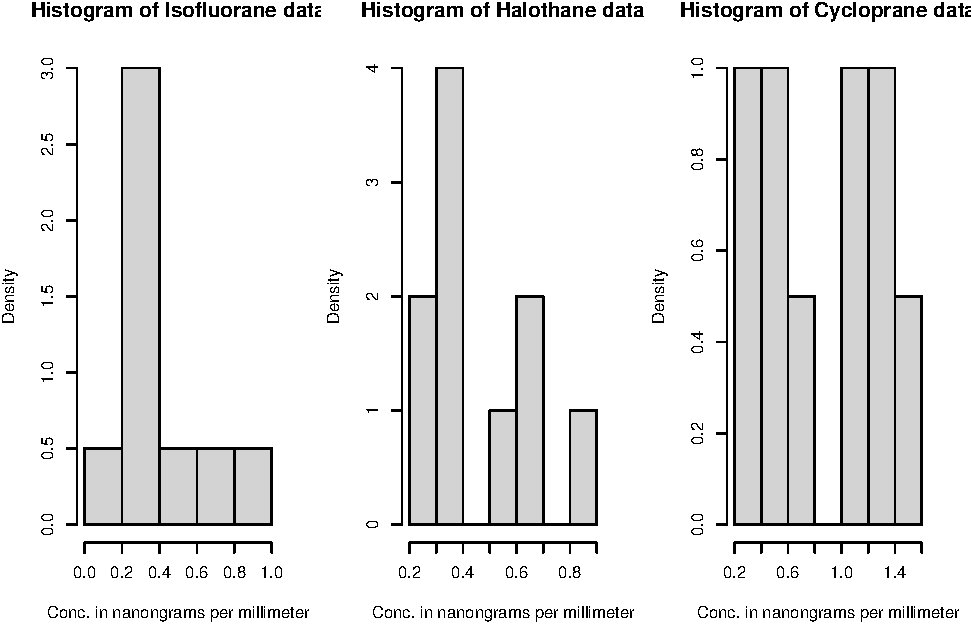
\includegraphics{assignment1_group75_final_files/figure-latex/unnamed-chunk-16-1.pdf}

Looking visually at histograms, the data doesn't look to be distributed
normally across any variable.

\textbf{QQ-Plots}

\begin{Shaded}
\begin{Highlighting}[]
\FunctionTok{par}\NormalTok{(}\AttributeTok{mfrow=}\FunctionTok{c}\NormalTok{(}\DecValTok{1}\NormalTok{,}\DecValTok{3}\NormalTok{))}
\FunctionTok{qqnorm}\NormalTok{(Isofluorane,}\AttributeTok{main=}\StringTok{"QQ{-}Plot of Isofluorane data"}\NormalTok{)}
\FunctionTok{qqline}\NormalTok{(Isofluorane)}
\FunctionTok{qqnorm}\NormalTok{(Halothane,}\AttributeTok{main=}\StringTok{"QQ{-}Plot of Halothane data"}\NormalTok{)}
\FunctionTok{qqline}\NormalTok{(Halothane)}
\FunctionTok{qqnorm}\NormalTok{(Cyclopropane,}\AttributeTok{main=}\StringTok{"QQ{-}Plot of Cyclopropane data"}\NormalTok{)}
\FunctionTok{qqline}\NormalTok{(Cyclopropane)}
\end{Highlighting}
\end{Shaded}

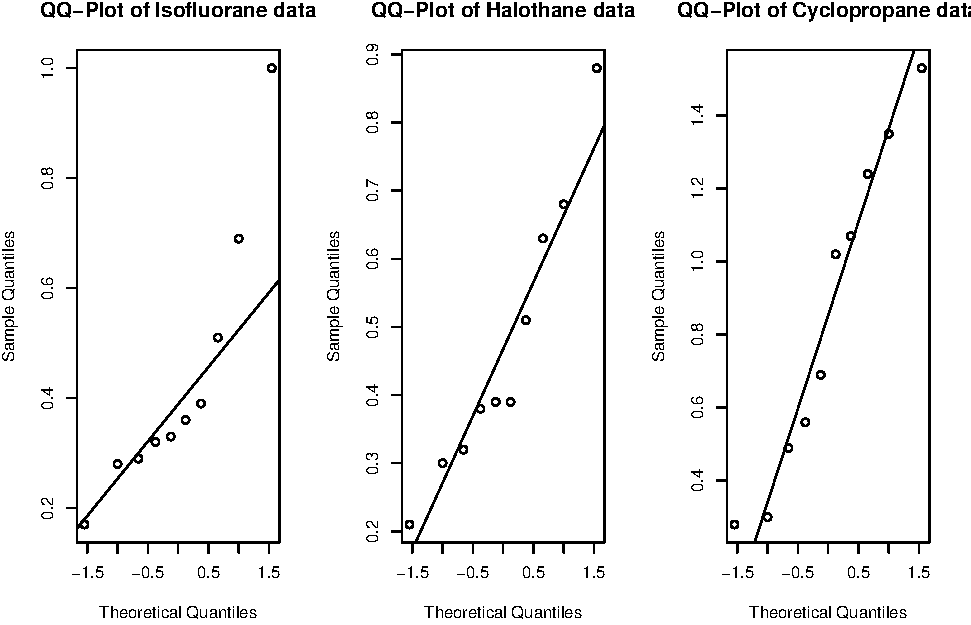
\includegraphics{assignment1_group75_final_files/figure-latex/unnamed-chunk-17-1.pdf}

QQ-Plots reveal a better picture of the normality and looking at it,
Halothane and Cyclopropane data look promising candidates for normality.

To confirm our inference, lets go through Shapiro-Wilk normality test.

\textbf{Shapiro-Wilk Normality Test}

\begin{Shaded}
\begin{Highlighting}[]
\FunctionTok{print}\NormalTok{(}\FunctionTok{shapiro.test}\NormalTok{(Isofluorane))}
\end{Highlighting}
\end{Shaded}

\begin{verbatim}
## 
##  Shapiro-Wilk normality test
## 
## data:  Isofluorane
## W = 0.831, p-value = 0.034
\end{verbatim}

\begin{Shaded}
\begin{Highlighting}[]
\FunctionTok{print}\NormalTok{(}\FunctionTok{shapiro.test}\NormalTok{(Halothane))}
\end{Highlighting}
\end{Shaded}

\begin{verbatim}
## 
##  Shapiro-Wilk normality test
## 
## data:  Halothane
## W = 0.923, p-value = 0.39
\end{verbatim}

\begin{Shaded}
\begin{Highlighting}[]
\FunctionTok{print}\NormalTok{(}\FunctionTok{shapiro.test}\NormalTok{(Cyclopropane))}
\end{Highlighting}
\end{Shaded}

\begin{verbatim}
## 
##  Shapiro-Wilk normality test
## 
## data:  Cyclopropane
## W = 0.933, p-value = 0.48
\end{verbatim}

Halothane and Cyclopropane data have p-values \textgreater{} 0.05, which
means we can accept the Null Hypothesis \(H_0\) that data is normally
distributed. On the other hand, Isofluorane data isn't normally
distributed as p-value \textless= 0.05.

\textbf{Final Answer}

On visual inspection, all 3 variables in dataset didn't look visually
normal using histogram inspection, but Halothane and Cyclopropane had
somewhat straight qq-plots (variation due to low number of
observations).

On closer inspection through Shapiro-Wilk Normality test, Isofluorane
proved to be not normally distributed at all but Halothane and
Cyclopropane concentrations were indeed normally distributed through the
dataset.

\hypertarget{b-2}{%
\paragraph{\texorpdfstring{\textbf{3B}}{3B}}\label{b-2}}

To check correlation between 2 normally distributed variables, we can
apply Pearson's test for correlation. From 3-A, we realise that variable
Isofluorane is not normally distributed. Therefore, we cannot use this
test to check for its correlation with Halothane.

In this case, we will use Spearman's rank test for correlation.

\begin{Shaded}
\begin{Highlighting}[]
\FunctionTok{print}\NormalTok{(}\FunctionTok{cor.test}\NormalTok{(Isofluorane,Halothane,}\AttributeTok{method=}\FunctionTok{c}\NormalTok{(}\StringTok{"spearman"}\NormalTok{)))}
\end{Highlighting}
\end{Shaded}

\begin{verbatim}
## Warning in cor.test.default(Isofluorane, Halothane, method = c("spearman")):
## Cannot compute exact p-value with ties
\end{verbatim}

\begin{verbatim}
## 
##  Spearman's rank correlation rho
## 
## data:  Isofluorane and Halothane
## S = 129, p-value = 0.54
## alternative hypothesis: true rho is not equal to 0
## sample estimates:
##     rho 
## 0.21885
\end{verbatim}

Since obtained \(\rho \neq 0\) , there might be some degree of positive
correlation between both variables in our data. But p-value of 0.54
indicates that Null-Hypothesis is significantly supported, hence true
\(\rho = 0\) and it indicates no correlation between values of
Isofluorane and Halothane. We need to note that p-value might not be
correct due to presence of ties (same-values) in a fairly small sample
size (10).

In 3-A, using Shapiro-Wilk Normality Test, it has already been concluded
that variable Isofluorane doesn't come from a normal distribution while
variable Halothane comes from a normal distribution.

\begin{Shaded}
\begin{Highlighting}[]
\FunctionTok{print}\NormalTok{(}\FunctionTok{ks.test}\NormalTok{(Isofluorane,Halothane))}
\end{Highlighting}
\end{Shaded}

\begin{verbatim}
## Warning in ks.test(Isofluorane, Halothane): cannot compute exact p-value with
## ties
\end{verbatim}

\begin{verbatim}
## 
##  Two-sample Kolmogorov-Smirnov test
## 
## data:  Isofluorane and Halothane
## D = 0.3, p-value = 0.76
## alternative hypothesis: two-sided
\end{verbatim}

Using Kolmogorov-Smirnov Tests, we get a P-value of 0.76 indicating that
2 variable distributions might be similar. Again, due to low sample size
and presence of ties, the calculated value of p-value can have some
inaccuracies.

\begin{Shaded}
\begin{Highlighting}[]
\FunctionTok{print}\NormalTok{(}\FunctionTok{paste}\NormalTok{(}\StringTok{"Length of datasamples : "}\NormalTok{,}\FunctionTok{length}\NormalTok{(Isofluorane),}\FunctionTok{length}\NormalTok{(Halothane),}\FunctionTok{length}\NormalTok{(Cyclopropane)))}
\end{Highlighting}
\end{Shaded}

\begin{verbatim}
## [1] "Length of datasamples :  10 10 10"
\end{verbatim}

Since size of data sample is small (10\textless30) and from 3-A we know
1st column does not follow normal distribution, we can say that
Permutation tests are applicable in this case.

\hypertarget{c-2}{%
\paragraph{\texorpdfstring{\textbf{3C}}{3C}}\label{c-2}}

Performing ANOVA test,

\begin{Shaded}
\begin{Highlighting}[]
\CommentTok{\#Creating DataFrame}

\NormalTok{df }\OtherTok{=} \FunctionTok{data.frame}\NormalTok{(}\AttributeTok{Concentration=}\FunctionTok{as.vector}\NormalTok{(}\FunctionTok{as.matrix}\NormalTok{(dogs\_data)),}\AttributeTok{An\_Type=}\FunctionTok{factor}\NormalTok{(}\FunctionTok{rep}\NormalTok{(}\DecValTok{1}\SpecialCharTok{:}\DecValTok{3}\NormalTok{,}\AttributeTok{each=}\DecValTok{10}\NormalTok{)))}

\CommentTok{\#Creating Linear Model}
\NormalTok{mod\_1 }\OtherTok{=} \FunctionTok{lm}\NormalTok{(Concentration }\SpecialCharTok{\textasciitilde{}}\NormalTok{ An\_Type, }\AttributeTok{data=}\NormalTok{df)}

\CommentTok{\#Performing ANOVA Test}
\FunctionTok{anova}\NormalTok{(mod\_1)}
\end{Highlighting}
\end{Shaded}

\begin{verbatim}
## Analysis of Variance Table
## 
## Response: Concentration
##           Df Sum Sq Mean Sq F value Pr(>F)  
## An_Type    2   1.08   0.540    5.35  0.011 *
## Residuals 27   2.73   0.101                 
## ---
## Signif. codes:  0 '***' 0.001 '**' 0.01 '*' 0.05 '.' 0.1 ' ' 1
\end{verbatim}

\begin{Shaded}
\begin{Highlighting}[]
\CommentTok{\#Printing output parameters of our Linear Model}
\FunctionTok{summary}\NormalTok{(mod\_1)}
\end{Highlighting}
\end{Shaded}

\begin{verbatim}
## 
## Call:
## lm(formula = Concentration ~ An_Type, data = df)
## 
## Residuals:
##    Min     1Q Median     3Q    Max 
## -0.573 -0.161 -0.079  0.200  0.677 
## 
## Coefficients:
##             Estimate Std. Error t value Pr(>|t|)    
## (Intercept)    0.434      0.101    4.32  0.00019 ***
## An_Type2       0.035      0.142    0.25  0.80727    
## An_Type3       0.419      0.142    2.95  0.00650 ** 
## ---
## Signif. codes:  0 '***' 0.001 '**' 0.01 '*' 0.05 '.' 0.1 ' ' 1
## 
## Residual standard error: 0.318 on 27 degrees of freedom
## Multiple R-squared:  0.284,  Adjusted R-squared:  0.231 
## F-statistic: 5.35 on 2 and 27 DF,  p-value: 0.011
\end{verbatim}

Looking at the p-value from the summary of the linear model and ANOVA
test table, P-value = 0.011 \textless{} 0.05, we can definitely say that
One Way ANOVA test determines that the type of drug has a significant
effect on the concentration of plasma epinephrine.

\begin{Shaded}
\begin{Highlighting}[]
\FunctionTok{confint}\NormalTok{(mod\_1)}
\end{Highlighting}
\end{Shaded}

\begin{verbatim}
##                2.5 %  97.5 %
## (Intercept)  0.22788 0.64012
## An_Type2    -0.25650 0.32650
## An_Type3     0.12750 0.71050
\end{verbatim}

In the confidence level of 95\%,

Estimated concentration of each type of drug is :

Isofluorane : 22.79 \% to 64.01\%

Halothane : 0.0\% to 32.65 \% (ignoring the negative Concentration value
as it is not semantically possible)

Cyclopropane : 12.75\% to 71.05\%

\hypertarget{d-2}{%
\paragraph{\texorpdfstring{\textbf{3D}}{3D}}\label{d-2}}

Performing the Kruskal-Wallis test :

\begin{Shaded}
\begin{Highlighting}[]
\NormalTok{Concentration }\OtherTok{=}\NormalTok{ df}\SpecialCharTok{$}\NormalTok{Concentration}
\NormalTok{Anesthesia\_Type }\OtherTok{=}\NormalTok{ df}\SpecialCharTok{$}\NormalTok{An\_Type}
\FunctionTok{kruskal.test}\NormalTok{(Concentration }\SpecialCharTok{\textasciitilde{}}\NormalTok{ Anesthesia\_Type, }\AttributeTok{data =}\NormalTok{ df)}
\end{Highlighting}
\end{Shaded}

\begin{verbatim}
## 
##  Kruskal-Wallis rank sum test
## 
## data:  Concentration by Anesthesia_Type
## Kruskal-Wallis chi-squared = 5.64, df = 2, p-value = 0.059
\end{verbatim}

The p-value given using Kruskal-Wallis Test comes out to be 0.059
(\textgreater{} 0.05). Hence the Null Hypothesis of this test is
accepted, meaning it considers the effect of type of drug insignificant
on the concentration of plasma epinephrine in the blood.

This is in contrast with the inference deduced using ANOVA test,
although not by a far off margin since the p-value is very close 0.05 in
case of Kruskal-Wallis test as well. This might be due to the nature of
distribution as Kruskal-Wallis is a rank-based test, while ANOVA uses
the nature of distribution such as Mean to compute the effect of the
independent variable on the dependent variable. In our case, the first
variable (Isofluorane) doesn't come from a standard normal distribution,
while the other 2 variables do. Hence, Kruskal-Wallis might be a better
representation of the effect of drugs on the plasma epinephrine
concentration in our case since it is a non-parametric test.

\hypertarget{question-4}{%
\subsection{Question 4}\label{question-4}}

Hemoglobin in trout

\hypertarget{a-3}{%
\paragraph{\texorpdfstring{\textbf{4A}}{4A}}\label{a-3}}

\hypertarget{b-3}{%
\paragraph{\texorpdfstring{\textbf{4B}}{4B}}\label{b-3}}

Check for normality before using ANOVA-test. The data comes from normal
distributions, since both the histogram and QQ-plot show a normally
distributed graph. Besides, the shapiro-wilk test gives a p-value of
0.526 which is above 0.05 and therefore suggests that the data comes
from normal distribution.

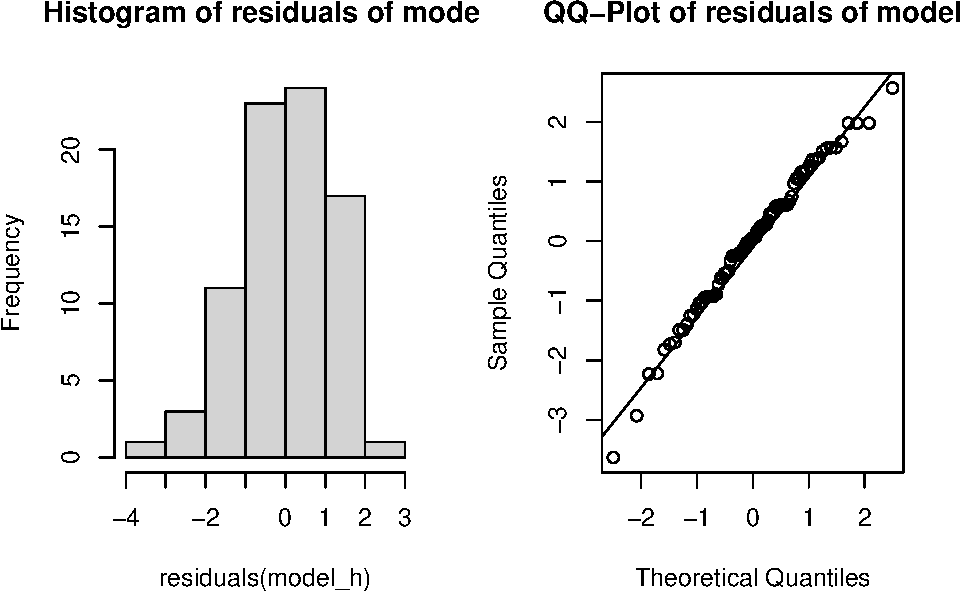
\includegraphics{assignment1_group75_final_files/figure-latex/unnamed-chunk-27-1.pdf}

From the two-way ANOVA test, we can see that the treatment variable
`rate' has a significant effect on hemoglobin, since the p-value is
below 0.05. However, the block variable `method' does not have a
significant effect on hemoglobin since it's p-value is 0.216, which is
above 0.05. The p-value for rate:method is 0.377, which means that there
is no evidence for interaction.

\hypertarget{c-3}{%
\paragraph{\texorpdfstring{\textbf{4C}}{4C}}\label{c-3}}

The factor `rate' has the greatest influence on hemoglobin, since rate
has a significant effect on hemoglobin and method does not have a
significant effect on hemoglobin. However, since there is no interaction
between rate and method, we have to remove the interaction term from the
model and create an additive model where there is no interaction. Still,
only the variable rate has a main effect on hemoglobin, and not the
variable `method'.

The combination of rate 2 and method B leads to the highest mean of
hemoglobin

Estimate the mean hemoglobin value for rate 3 by using method A.

The mean of rate 3 and method A is 9.03

Rate 2 leads to the highest mean of hemoglobin.

\hypertarget{d-3}{%
\paragraph{\texorpdfstring{\textbf{4D}}{4D}}\label{d-3}}

The results from the one-way ANOVA are exactly equal to the results of
the two-way ANOVA. In both tests the effect of each rate on hemoglobin
is tested and therefore, it is unnecessary to do the one-way ANOVA.

\hypertarget{question-5}{%
\subsection{Question 5}\label{question-5}}

\hypertarget{a-4}{%
\paragraph{\texorpdfstring{\textbf{5A}}{5A}}\label{a-4}}

To perform a three-way ANOVA test, we need to check normality. This is
done by creating a QQ-plot and histogram of the residuals of the data.
Additionally, the Shapiro-Wilk test was performed. The line in the
QQ-plot looks linear and the distribution of the histogram can come from
a normal distribution. Besides, the Shapiro-Wilk test had a p-value
larger than 0.05 which means that the data comes from normal
distribution. Therefore, a three-way ANOVA can be performed.

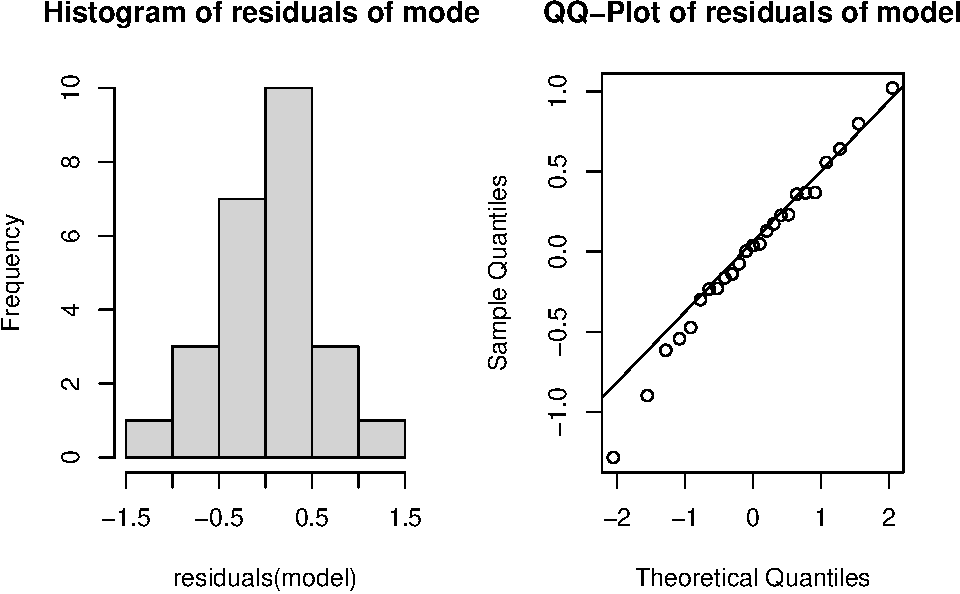
\includegraphics{assignment1_group75_final_files/figure-latex/unnamed-chunk-34-1.pdf}

Starter 1 is the intercept, which has a p-value of less than 0.05.
Therefore there is a significant effect of starter 1 on acidity. While
starter 2 has a p-value of 0.754, and therefore has no significant
effect on acidity.

\hypertarget{b-4}{%
\paragraph{\texorpdfstring{\textbf{5B}}{5B}}\label{b-4}}

Insignificant block variables, are variables that have a p-value larger
than 0.05. So this is the block variable position, which has a p-value
of 0.411

After deleting the block variable position, starter 4 leads to a
significantly different acidity.

\hypertarget{c-4}{%
\paragraph{\texorpdfstring{\textbf{5C}}{5C}}\label{c-4}}

In the Friedman test the data does not need to come from a normal
distribution, but it can also be used when the data comes from a normal
distribution, like in this case. Instead of using the mean of the groups
in an ANOVA test the Friedman makes use of ranks. However, this
difference does not make any difference in the use of this test.
Therefore, the Friedman test can also be used in this application to
test whether there is an effect of starter on acidity. However, the
Friedman test is not necessary when the ANOVA test has already been
performed.

\hypertarget{d-4}{%
\paragraph{\texorpdfstring{\textbf{5D}}{5D}}\label{d-4}}

Formula mixed effects is acidity \textasciitilde{}
starter+(1\textbar batch). Where the 1\textbar batch is used to make
from the block variable `batch' a random effect variable.

When using the fixed effects model the variables 1 and starter 4 had a
significant effect on acidity. In the mixed effects model variables
starter 1, starter 3, starter 4 had a significant effect on acidity. So,
with the mixed effect model, more starters have a significant effect on
acidity.

\end{document}
